\documentclass [a4paper, 11pt, twoside] {article}

\usepackage [utf8] {inputenc}
\usepackage[french]{babel}
\usepackage[T1]{fontenc}
\usepackage{amssymb}
\usepackage{amsthm}
\usepackage{a4wide}
\usepackage{graphicx}

\begin{document}

\theoremstyle{plain}
\newtheorem{Thm}{Théorème}

\section{Approche analytique}

Cette approche pour créer des ensembles aléatoires (désignés par $Q$) qui partagent la même distribution que celle des nombres
premiers, est basée sur un théorème (théorème \ref{theorem}) issu de ... . 

\begin{Thm}
\label{theorem}
	L'hypothèse de Reimann est équivalente à l'assertion 
	\[
	\forall \ n \geqslant 11, \ |p_{n} - ali(n) | < \frac{1}{\pi} \sqrt{n} \log^{5/2}(n) 
	\]
	où $p_{n}$ représente le n-ième nombre premier.
\end{Thm}

Les onze premiers éléments d'un ensemble $Q$ sont choisis arbitrairement. 
Pour $ n > 11 $, voici la méthode de sélection  de l'élément $q_{n} \in Q$: 
\begin{itemize}
	\item on pose $ a = \max \left\{ q_{n-1} ,\lceil{ali(n) - \frac{1}{\pi} \sqrt{n} \log^{5/2}(n) \rceil} \right\}$ 
	(où $\lceil x \rceil$ désigne la partie entière supérieure de $x$);
	\item on pose $ b = \lfloor ali(n) + \frac{1}{\pi} \sqrt{n} \log^{5/2}(n) \rfloor $
	(où $\lfloor x \rfloor$ désigne la partie entière inférieure de $x$);
	\item $ q_{n} $ est choisi aléatoirement entre a et b. 
\end{itemize}

On peut désormais définir $ \sigma : [0, \infty [$  $\rightarrow \mathbb{R} $, $ x \mapsto \# \left\{ n \in Q : n < x \right\} $. Nous parlerons systématiquement de  la fonction $\sigma$ alors que cette fonction n'est bien entendu pas unique, elle dépend à chaque fois de l'ensemble aléatoire $Q$ sur lequel on travail. Cependant, nous avons pu remarquer que  les différentes fonctions $\sigma$ sont souvent très proches les unes des autres. À titre d'exemple,  pour un grand nombre d'ensembles aléatoires $Q$, nous avons calculé $\sigma(1000)$. Pour $45 \%$ des ensembles, $\sigma(1000) = 148$ et parmis $42\%$ d'entre eux, $\sigma(1000) = 147$.

Afin de visualiser  $\sigma(x)$ en la comparant à $\pi(x)$ et $\frac{x}{\log(x)}$, voici leur graphe respectif : 

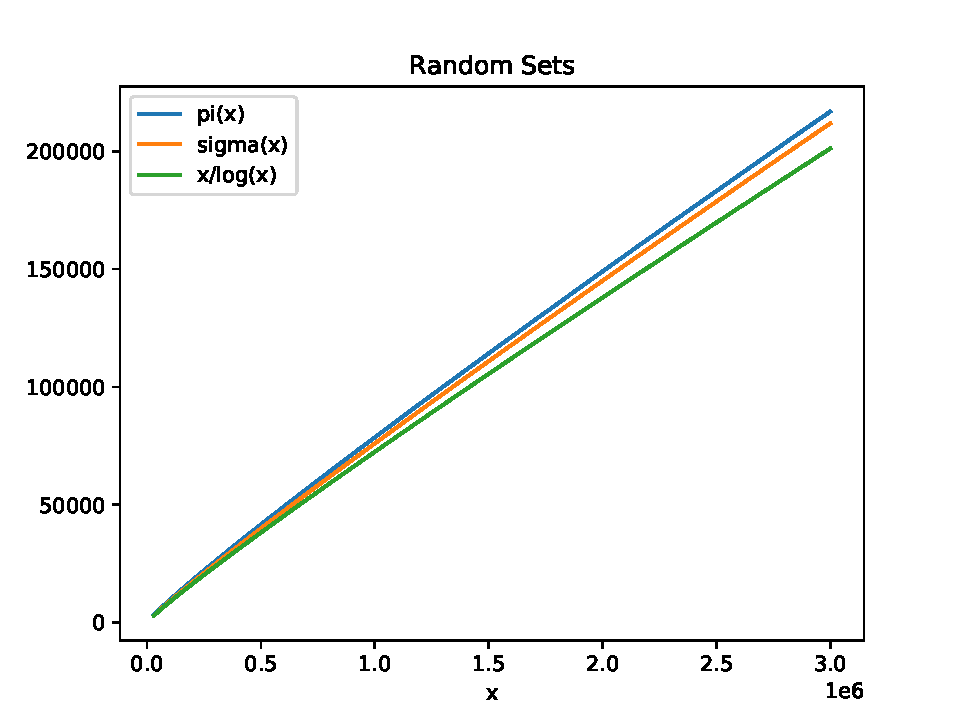
\includegraphics{approche_analytique_sets_2.pdf}



\end{document}